\documentclass[11pt,a4paper]{article}
\usepackage[margin=2.3cm]{geometry}
\usepackage{amsmath,amssymb}
\usepackage{graphicx}
\usepackage{booktabs}
\usepackage{array}
\usepackage{xcolor}
\usepackage{enumitem}
\usepackage[hidelinks]{hyperref}
\usepackage{caption}
\emergencystretch=1.5em
\captionsetup{font=small,labelfont=bf,width=.92\textwidth}
\setlength{\parskip}{4pt plus 1pt}
\setlength{\parindent}{0pt}

\newcommand{\code}[1]{\texttt{#1}}
\newcommand{\neff}{n_{\mathrm{eff}}}
\newcommand{\chigeo}{\chi_{\mathrm{geo}}}
\newcommand{\Pisurr}{\Pi}
\newcommand{\EMA}{\operatorname{EMA}}

\title{Order parameter and mechanism of the RBLapSum
\code{through\_rank\_kappa} instability\\[2pt]
\large Research note: one-step score-scale dynamics}
\author{}
\date{2026-09-16/17. Follow-up to the kappa stability investigation.}

\begin{document}
\maketitle
\vspace{-2em}
\tableofcontents

\section{Purpose and summary of conclusions}

The previous investigation (\code{docs/rblapsum-kappa-stability-neutral.tex})
introduced the geometric indicator
\[
\chigeo = \frac{b}{2T\delta}
\]
and used it as an empirical instability proxy. This note treats that proxy as
a hypothesis and asks four questions: whether \(\chigeo\) is the right control
parameter (H1); whether the dimensionless surrogate gain
\(\Pisurr = \lVert L_\kappa D_z\rVert_F^2\) is a better geometric quantity
(H2); what dynamical mechanism produces score-inflation bursts (H3); and
whether \(\neff \to 1\) is a cause or a late-stage consequence (H4).


The measured answers, stated fully in the final sections:

\begin{itemize}[leftmargin=1.4em]
\item \textbf{H1 (proxy): supported.} \(\chigeo\) is not
reparameterization-invariant; an exact score-units transformation leaves the
training dynamics identical while scaling \(\chigeo\) arbitrarily, and
within a fixed \((K,T)\) row \(\chigeo\) has no prospective signal
(AUC \(\approx\) 0.46).
\item \textbf{H2 (surrogate gain): supported as the gain measure.}
\(\Pisurr = \lVert L_\kappa D_z\rVert_F^2\) is dimensionless, invariant,
predicts the realized gradient gain (rank correlation 0.97 vs 0.52 for
\(\chigeo\)), and its dense-boundary approximation \(b^2/(4T\delta)\) holds
within a factor of two in healthy states.
\item \textbf{H3 (coupling to scale): supported in the diffusion/heating
form.} The signed surrogate drift is restoring at the dangerous states; the
destabilizing coupling is the second-order heating of the scale by large
parameter steps (even under sign flip of the gradient, \(\propto\)
lr\(^2\), and at hot states deterministic rather than minibatch noise).
Instability occurs where heating exceeds the restoring drift.
\item \textbf{H4 (\(\neff \to 1\) late-stage): supported with a
refinement.} The one-feature limit does null the corrected gradient
(measured \(\Pisurr = 0\)), but near-degenerate blocks continue to pump;
post-collapse growth stops only when the support gradient is disabled, and
kernel broadening after the collapse makes things worse.
\item \textbf{Practical controller variables:} per-block window population
(\(\neff\), the best within-row early warning, AUC 0.75) for the fast
guard; \(\Pisurr\) as the portable pressure gauge; support-gradient
shutdown, not kernel broadening, as the correct emergency action after a
collapse.
\end{itemize}


\section{Definitions}

All quantities are computed per layer from the candidate set of the gate
(the top \(K{+}J\) features by score).

\begin{itemize}[leftmargin=1.4em]
\item Scores \(s_i = |z_i|\); boundary \(b = \max(b_0, s_{(K+1)})\); kernel
\(\kappa_i = e^{-|s_i - b|/T}/(2T)\); \(Z = \sum_i \kappa_i\);
\(\neff = Z^2 / \sum_i \kappa_i^2\); local spacing
\(\delta = (s_{(K-3)} - s_{(K+5)})/8\).
\item The kappa-corrected support gradient, written with
\(D_\kappa = \mathrm{diag}(\kappa)\) and
\(L_\kappa = D_\kappa - \kappa\kappa^{\top}/Z\), is
\[
g_s = -\,L_\kappa\, w,
\qquad w_i = -u_i z_i,
\qquad u_i = \partial L/\partial y_i ,
\]
equivalently \(g_s = L_\kappa D_z u\) up to the sign convention.
\item Exact surrogate gain
\(\Pisurr = \lVert L_\kappa D_z \rVert_F^2\), computed per token from the
diagonal-minus-rank-one structure:
\[
\Pisurr \;=\; \sum_j z_j^2 \kappa_j^2
\Bigl[\bigl(1 - \kappa_j/Z\bigr)^2 + \bigl(\textstyle\sum_i \kappa_i^2 -
\kappa_j^2\bigr)/Z^2\Bigr].
\]
\(\Pisurr\) is dimensionless (each factor \(\kappa_j z_j\) is a pure number),
unlike \(\chigeo\), which carries units of 1/score. The dense-boundary
approximation tested below is \(\Pisurr \approx b^2/(4T\delta)\).
\item Empirical gain \(G_{\mathrm{emp}} = \lVert g_s\rVert^2 / \lVert
u\rVert^2\) over candidates.
\item Scale statistics on a fixed evaluation batch:
\(R_{\mathrm{all}} = \mathrm{RMS}_i(s_i)\) over all features,
\(R_K\) = mean of the top-\(K\) scores, and \(b\); the scale variable is
\(x = \log R\).
\item One-step counterfactual updates from a saved model+optimizer state:
branches \emph{null} (zero gradient), \emph{task} (support gradient
disabled), \emph{full}, and their antithetic negatives. The saved Adam-type
state replays momentum on every branch, and any parameter perturbation
inflates \(R\) at second order (heating), so the signed drift is the
antithetic odd part
\(\mu = \tfrac12\,\mathbb{E}[\Delta x(+G) - \Delta x(-G)]\)
and the heating is the even part relative to the null step. The support
contribution is \(\mathrm{odd}(\mathrm{full}) - \mathrm{odd}(\mathrm{task})\);
raw-gradient decomposition \(G_{\mathrm{full}} = G_{\mathrm{task}} +
G_{\mathrm{supp}}\) is exact (verified; identical RNG, no stochastic layers),
while optimizer steps are nonlinear in the gradient and are always reported
as separate branch counterfactuals.
\end{itemize}

\section{Experiments performed}

\begin{enumerate}[leftmargin=1.6em]
\item \textbf{Checkpoint library.} Thirteen states spanning: calm
(\(T{=}2\)), stable (\(k32/T1\)), a marginal survivor around a recoverable
burst (\(k32\,j224\,T0.5\) at steps 2000/4000/6000), marginal states of runs
that later died (\(k32\,j480\,T0.5\); \(k64\,j448\,T1\)), and a post-collapse
state (\(k32\,j480\,T0.1\)). All checkpoints carry full optimizer state.
State-class labels describe the run's eventual fate; except for the
post-collapse state, every checkpoint is healthy at measurement time (in
particular, ``pre-death'' means a healthy step-2000 state of the run that
destabilized at step 3940).
\item \textbf{One-step drift/diffusion} (16 batches per state, five branch
steps per batch, per-layer \(\Delta \log R\) on a fixed evaluation batch).
\item \textbf{Surrogate gain and radial structure} per state and layer:
\(\Pisurr\), \(b^2/(4T\delta)\), \(\chigeo\), \(\neff\), \(G_{\mathrm{emp}}\),
the radial projection \(r_{\mathrm{supp}} = -s^{\top} g_s^{(z)} / s^{\top}s\),
\((s-b)^{\top}L_\kappa w\), \(\operatorname{Cov}_q(s{-}b, w)\), and a
permutation null (48 shuffles of \(w\) among candidates per token).
\item \textbf{Scale-response curves} \(F(\alpha)\): a gate-level
function-preserving rescaling \(z \to \alpha z\) (output divided by
\(\alpha\)) leaves the forward and the task gradient exactly unchanged
(unit-tested and verified in the measurements) while the surrogate sees an
\(\alpha\)-times score excursion at fixed \(T\); drift branches are measured
at \(\alpha \in \{0.5, 0.75, 1, 1.25, 1.5, 2, 3\}\) at four reference states.
\item \textbf{Score-units reparameterization}: \(\alpha = c\) together with
\(T \to cT\) must leave all gradients invariant while \(\chigeo \to
\chigeo/c\).
\item \textbf{Drift vs.\ heating scaling}: learning-rate multipliers
\(\{0.5, 1, 2\}\) and half batch size at three states.
\item \textbf{Counterfactual continuations} from a marginal \(k96/T1\) state
and from the post-collapse \(T{=}0.1\) state: normal replicas (three seeds),
support gradient disabled from the start or at a boundary-inflation trigger,
kernel broadened (\(T \times 3\), or \(T \times 30\) post-collapse) from the
start or at the trigger.
\item \textbf{Prospective order-parameter comparison} on 148
checkpoint-states from 18 earlier fixed-\(T\) runs: does a quantity measured
at step \(r\) predict a boundary burst in \((r, r{+}H]\), pooled and within
\((K,T)\) rows.
\end{enumerate}


\section{Results 1: the reparameterization test (H1)}

The gate-level reparameterization \((s, z, b, T) \to (c s, c z, c b, c T)\)
leaves the forward function and every parameter gradient invariant. This is
proved exactly in unit tests (float32, single gate) and confirmed on full
checkpoints: at \(c = 0.5\) and \(c = 2\) (both exact in floating point) the
training loss is unchanged to all printed digits and the worst relative
parameter-gradient difference is \(2\times10^{-3}\)--\(6\times10^{-3}\),
attributable to bf16 accumulation order. At \(c = 3\) (inexact mantissa
scaling) near-tied scores reorder in bf16 and the candidate sets change,
which shifts the loss by \(10^{-3}\); this is a numerics artifact, not a
violation of the invariance.

Under the same transformation \(\chigeo \to \chigeo/c\) (measured: layer-4
value 54.1 at \(c{=}1\), 27.0 at \(c{=}2\), 18.1 at \(c{=}3\)), while
\(\Pisurr\) is invariant. Identical training dynamics with different
\(\chigeo\) values means a universal numerical threshold in \(\chigeo\)
cannot be fundamental.

\textbf{H1 verdict: supported.} \(\chigeo\) is an empirical proxy. It
separates \((K,T)\) rows because it co-moves with the true geometry, but it
is not reparameterization-invariant, and (Results~5) it carries no
within-row temporal signal.

\section{Results 2: the surrogate gain \texorpdfstring{$\Pi$}{Pi} (H2)}

Across 96 layer-states (12 checkpoints \(\times\) 8 blocks, excluding the
post-collapse state), the exact \(\Pisurr\) predicts the realized gradient
gain \(G_{\mathrm{emp}}\) with rank correlation \(0.97\); \(\chigeo\)
reaches \(0.52\). The dense-boundary approximation
\(\Pisurr \approx b^2/(4T\delta)\) holds within a factor of about two at
the mid-depth blocks of healthy states and fails, as expected, when the
boundary region degenerates (factor 10 during late inflation; factor
\(10^{4}\) post-collapse). It can also \emph{over}estimate by orders of
magnitude at individual blocks whose local rank spacing collapses
(near-tied scores make \(\delta \to 0\) while the exact \(\Pisurr\)
stays moderate) --- visible as the rightmost points of
Fig.~1; where it matters, the exact \(\Pisurr\) should be used.

\begin{figure}[h]\centering
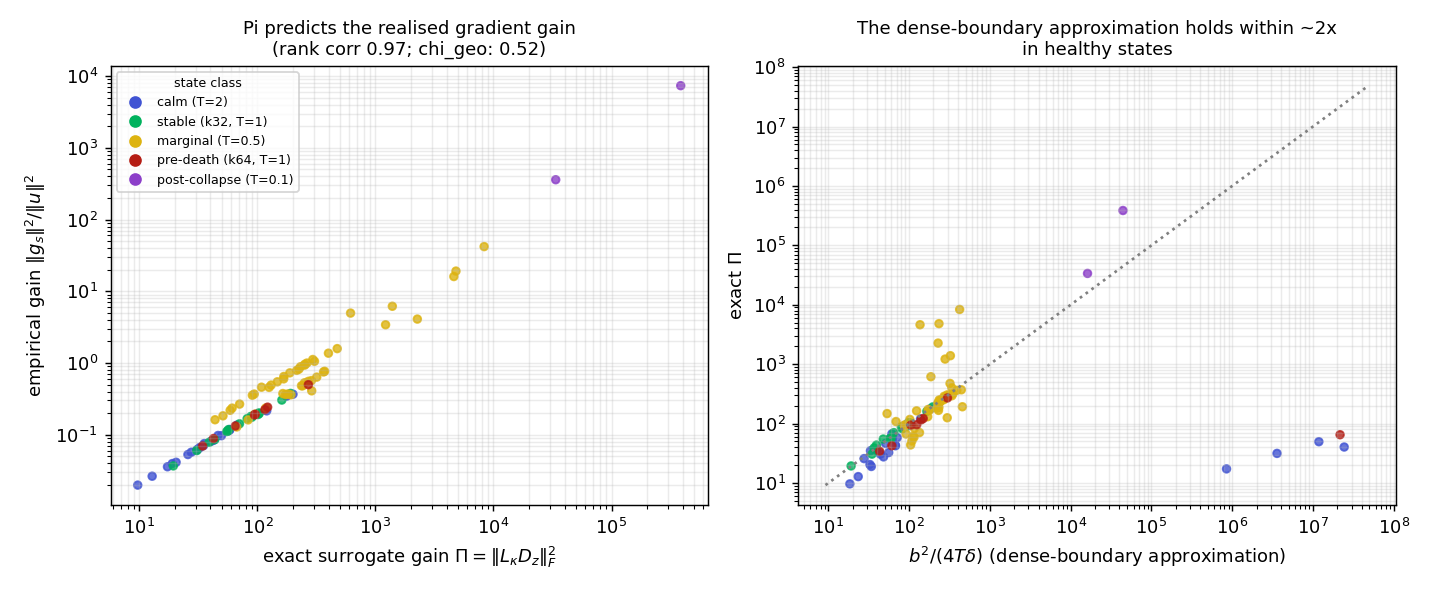
\includegraphics[width=.9\textwidth]{figures/sdn_Pi.png}
\caption{Left: exact \(\Pisurr\) against the realized gain
\(\lVert g_s\rVert^2/\lVert u\rVert^2\) across states and blocks. Right:
exact \(\Pisurr\) against the dense-boundary approximation. Each point is
one (checkpoint, block) pair; color encodes the checkpoint's state class:
calm (\(T{=}2\)), stable (\(k32/T1\)), marginal (\(T{=}0.5\)),
pre-death (\(k64/T1\)), post-collapse (\(T{=}0.1\)). The class labels
refer to the run's eventual fate, not to the condition at measurement
time: ``pre-death'' points come from a checkpoint (step 2000) at which the
run was still fully healthy but destabilized about 1{,}900 steps later;
only ``post-collapse'' points are measured after a collapse. No averaging
across blocks is performed --- each checkpoint contributes eight points,
one per block. The training step is the checkpoint step of the library
state (2000 for most states; 4000/6000 for the additional \(T{=}0.5\)
checkpoints; 10000 for one calm and one stable state). Within a point,
\(\Pisurr\) is the token mean over the fixed evaluation batch and
\(G_{\mathrm{emp}}\) the token mean over one training microbatch.}
\end{figure}

The predicted \(K\)- and \(T\)-ratios from the earlier report are
reproduced by the approximation
(\(\Pi_{\mathrm{approx}}(k64,T1)/\Pi_{\mathrm{approx}}(k32,T1) = 1.66\) at
step 2000, in the predicted 1.6--2.25 range) but compressed in the exact
value (ratio 1.09), because the exact \(\Pisurr\) weights the true kernel
and \(z\) profile rather than a uniform dense boundary.

\textbf{H2 verdict: supported as a gain measure.} \(\Pisurr\) is
dimensionless, reparameterization-invariant, and is the correct predictor
of how much gradient the surrogate injects. Whether large \(\Pisurr\)
implies instability is a separate question (H3).

\section{Results 3: signed drift versus heating (H3)}

\begin{figure}[h]\centering
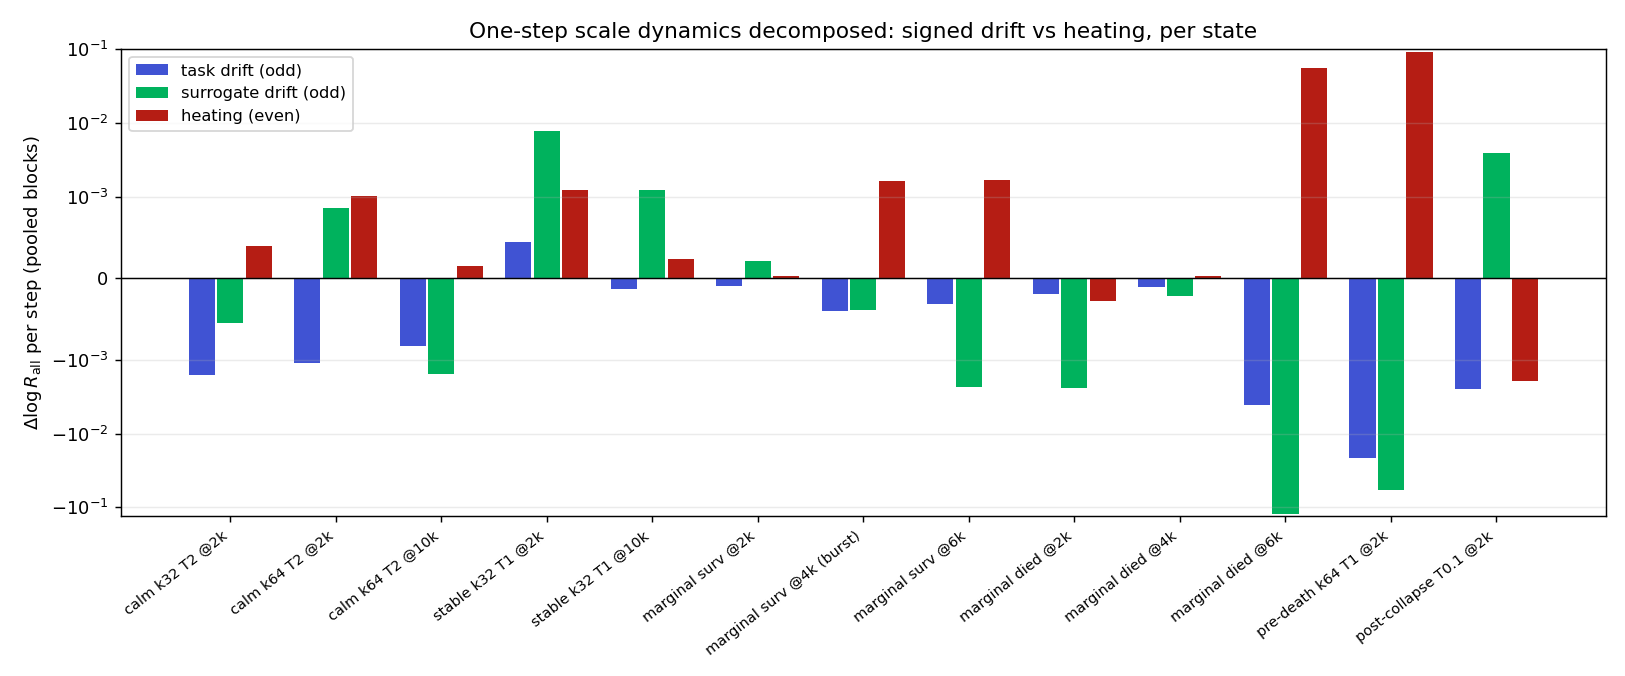
\includegraphics[width=\textwidth]{figures/sdn_decomposition.png}
\caption{One-step change of \(\log R_{\mathrm{all}}\) per training step,
decomposed into signed task drift, signed surrogate drift (antithetic odd
parts) and heating (even part), pooled over blocks, at thirteen states.}
\end{figure}

Three facts emerge.

\begin{enumerate}[leftmargin=1.6em]
\item \textbf{The signed surrogate drift is not the runaway force.} At the
state 1{,}940 steps before the \(k64/T1\) death, the surrogate's odd part is
\emph{strongly restoring} (\(-5.7\times10^{-2}\) per step pooled;
\(-0.10\) at the worst block), and the task odd part is also restoring
(\(-2.2\times10^{-2}\)). The same holds during late inflation of the dying
\(T{=}0.5\) run.
\item \textbf{The dominant destabilizing term is heating}: the even,
sign-independent inflation of \(R\) produced by the sheer size of the
parameter step (\(\mathbb{E}[(z{+}\delta z)^2] > z^2\)). At the pre-death
state it reaches \(+9.2\times10^{-2}\) per step pooled and \(+0.18\) at the
worst block --- larger than the restoring drift. At calm and stable states
heating is 30--300 times smaller. The learning-rate sweep confirms the
identification: the odd parts scale approximately linearly with the step
size, the even part approximately quadratically
(Fig.~\ref{fig:lr}).
\item \textbf{The heating at the pre-death state is deterministic, not
minibatch noise}: halving the batch size leaves it unchanged
(\(+9.3\times10^{-2}\) vs \(+9.2\times10^{-2}\)) and its across-batch
variance is small. It is second-order overshoot of a large, structured
gradient, not gradient-variance diffusion. At the stable \(k32/T1\) state,
by contrast, the (much smaller) heating roughly doubles under batch
halving, i.e.\ there it \emph{is} mostly stochastic.
\end{enumerate}

\begin{figure}[h]\centering
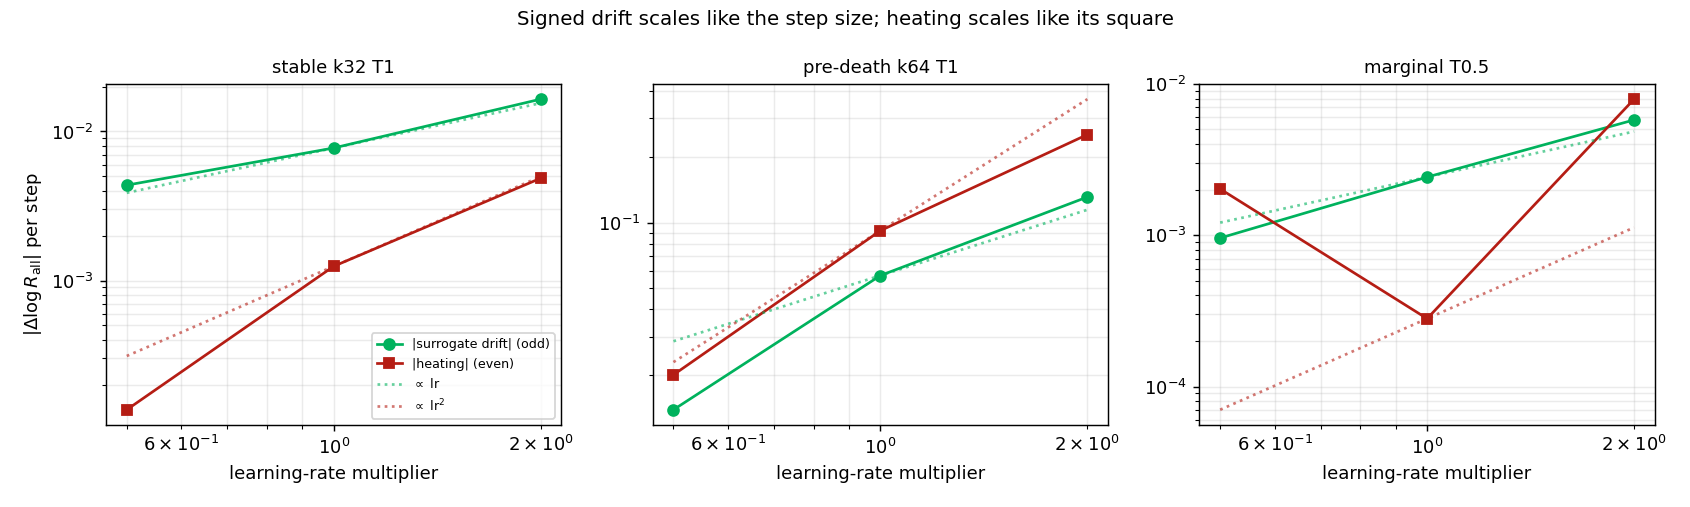
\includegraphics[width=\textwidth]{figures/sdn_lr_scaling.png}
\caption{\label{fig:lr}Drift and heating versus learning-rate multiplier at
three states, with reference slopes \(\propto\) lr and \(\propto\)
lr\(^2\).}
\end{figure}

The scale-response curves (Fig.~\ref{fig:falpha}) characterize the signed
part: the surrogate behaves as a spring in the gate-view scale. At the calm
\(k64/T2\) state it crosses zero near \(\alpha \approx 1.4\): it pushes the
scale up below that point and down above it --- a stable fixed point. At
the stable \(k32/T1\) state the spring pushes up over the whole measured
range with decreasing strength. The task drift is exactly
\(\alpha\)-independent by construction of the intervention, and measured to
be so, which also validates the isolation of the surrogate path.

\begin{figure}[h]\centering
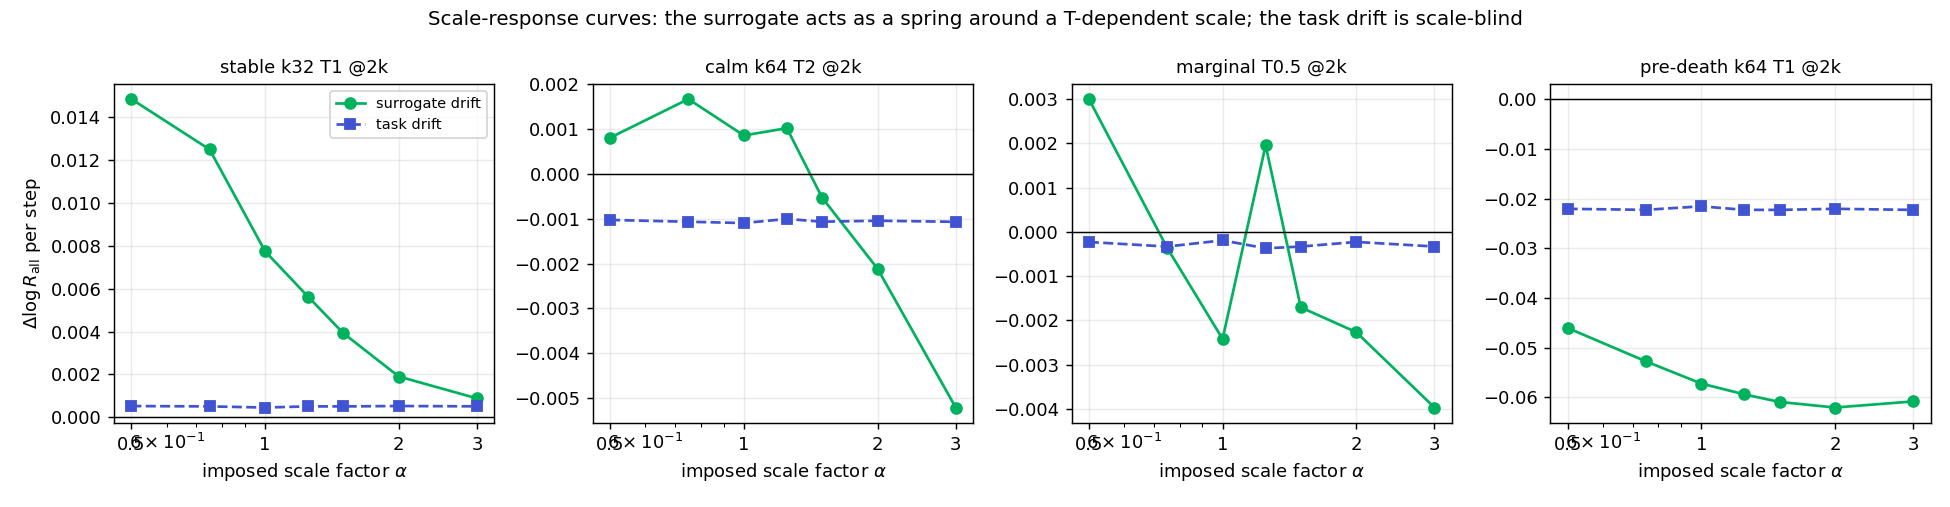
\includegraphics[width=\textwidth]{figures/sdn_Falpha.png}
\caption{\label{fig:falpha}Surrogate and task signed drift as functions of
an imposed function-preserving scale factor \(\alpha\) at four states.}
\end{figure}

The permutation test on the rank structure of \(w\) shows that the signed
radial component of the surrogate is statistically distinguishable from a
rank-shuffled null in most states (typically \(|z\text{-score}| \gtrsim
3\)--\(20\)), with an outward-aligned sign at the pre-death state
(\(+19.8\sigma\)) and inward-aligned signs at calm late states. The
magnitudes are, however, small compared with the heating term at the
dangerous states, so the sign structure sets the (mostly restoring)
spring, while the danger comes from the even term.

\textbf{H3 verdict: supported in its second form.} Large surrogate gain is
not sufficient for instability through a signed radial force; the coupling
to scale growth is primarily through second-order heating --- deterministic
step-size overshoot at the hot states --- opposed by a restoring drift.
Instability corresponds to heating exceeding restoration, layer by layer.


\section{Results 4: counterfactual interventions and the death arc (H4, causality)}

\begin{figure}[h]\centering
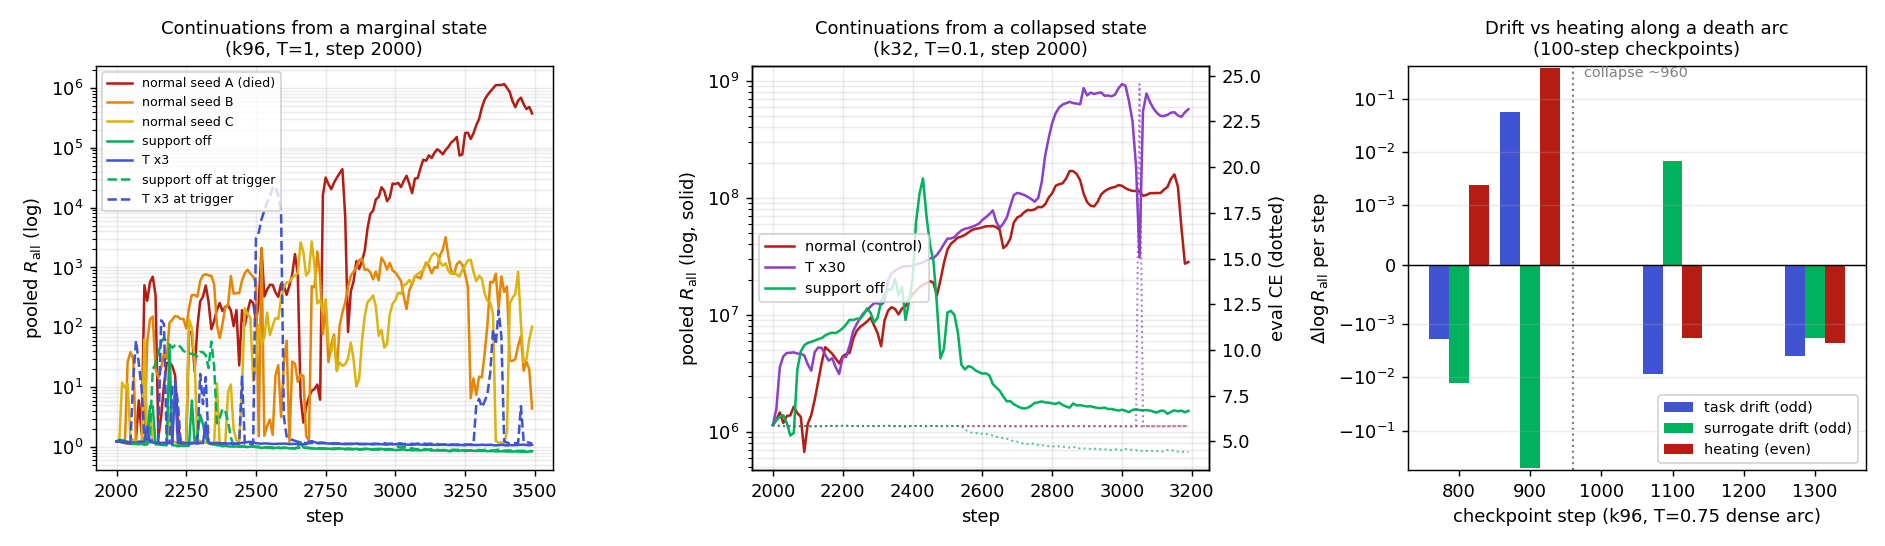
\includegraphics[width=\textwidth]{figures/sdn_interventions.png}
\caption{Left: continuations from a marginal \(k96/T1\) state (step 2000);
three normal seeds against support-off and \(T\times3\), applied from the
start (solid) or at a boundary-inflation trigger (dashed). Middle:
continuations from a collapsed \(T{=}0.1\) state; solid lines show scale,
dotted lines evaluation CE. Right: the one-step decomposition along a dense
death arc (\(k96, T{=}0.75\), checkpoints every 100 steps; collapse at
approximately step 960).}
\end{figure}

\textbf{From the marginal state} (\(k96/T1\), 1500-step continuations): all
three normal replicas show repeated scale bursts (excursions of one to three
orders of magnitude that mostly recover); one of three diverges terminally.
With the support gradient disabled, the trajectory is entirely calm and the
scale \emph{decreases} (task gradient alone is restoring, consistent with
the drift measurements); with \(T\times3\) the trajectory is calm at
unchanged scale and reaches the best evaluation CE of all branches (1.505
against 1.552--1.634). Both remedies also work when applied only at the
first trigger (boundary above three times its rolling median). The support
surrogate is therefore \emph{necessary} for burst initiation at this state.

\textbf{From the collapsed state} (\(T{=}0.1\), scale \(\sim10^6\)): the
control continues to inflate (\(\times25\) in 1200 steps) with CE frozen
near 5.8. Broadening the kernel (\(T\times30\)) \emph{accelerates} the
inflation (\(\times500\)): it re-populates the kernel window at a state
where some blocks have astronomically large \(\Pisurr\) (up to \(10^{12}\);
one block sits exactly at \(\neff = 1\) with \(\Pisurr = 0\), the measured
\(L_\kappa \to 0\) limit). Disabling the support gradient \emph{stops} the
inflation and the model begins to recover (CE \(5.93 \to 4.44\) in 1200
steps). Post-collapse scale growth is thus driven by the degenerate
surrogate, not by the task gradient.

\textbf{Along the dense death arc} (checkpoints every 100 steps): at 200
steps before collapse the decomposition is ordinary (restoring drift
\(-1.3\times10^{-2}\), heating \(+2.4\times10^{-3}\), already ten times the
calm level); at 60--100 steps before collapse both terms explode two orders
of magnitude (surrogate drift \(-0.50\), heating \(+0.37\) per step,
pooled) --- a violent tug-of-war whose balance tips block by block; after
collapse all terms are small again (kernel largely dead).

\textbf{H4 verdict: supported with a refinement.} \(\neff \to 1\) is a
late-stage phenomenon, and the strict one-feature limit does eliminate the
corrected support gradient (\(\Pisurr = 0\), measured). The refinement is
that the near-degenerate blocks that remain (\(\neff \approx 2\), very
large \(z\)) continue to pump scale: the late runaway is still
surrogate-driven, in its degenerate form. ``Loss of the stabilizing
distributed correction'' and ``continuing surrogate engine'' are therefore
both partially correct: the \emph{distributed} correction is lost, and what
remains of the surrogate is destabilizing.


\section{Results 5: prospective comparison of order parameters}

On 148 checkpoint-states from 18 earlier fixed-\(T\) runs (post-collapse
rungs excluded), predicting whether a boundary burst occurs within the next
\(H\) steps:

\begin{center}\small
\begin{tabular}{lcccccc}
\toprule
& \multicolumn{3}{c}{pooled AUC} & \multicolumn{3}{c}{within-row AUC} \\
\cmidrule(lr){2-4}\cmidrule(lr){5-7}
\(H\) & \(\chigeo\) & \(\Pi_{\mathrm{approx}}\) & \(1/\neff\)
      & \(\chigeo\) & \(\Pi_{\mathrm{approx}}\) & \(1/\neff\) \\
\midrule
1000 & 0.81 & \textbf{0.88} & 0.77 & 0.46 & 0.63 & \textbf{0.75} \\
2000 & 0.78 & \textbf{0.86} & 0.71 & 0.48 & 0.68 & \textbf{0.75} \\
4000 & 0.80 & \textbf{0.85} & 0.68 & 0.44 & 0.69 & \textbf{0.76} \\
\bottomrule
\end{tabular}
\end{center}

Pooled across configurations, \(\Pi_{\mathrm{approx}}\) dominates. Within a
fixed \((K,T)\) row --- the test that removes the between-row confound ---
\(\chigeo\) falls to chance, consistent with it being a row-level proxy,
while the smallest per-block \(\neff\) is the best temporal early-warning
signal (window depopulation precedes bursts), with \(\Pi\) second. Only the
three marginal rows contribute to the within-row comparison, so these
numbers are indicative rather than definitive.




\section{Results 5b: the fate map in \texorpdfstring{$\Pi$}{Pi}, per block and training step}

The analogue of the earlier report's dose--response figure, with the order
parameter replaced according to the present findings, and broken down over
blocks and training steps. Points are taken from pre-collapse checkpoints
only; the trajectory panel tracks the worst block of each run over
training; the dose--response panel plots the pre-onset burst rate against
the earliest healthy worst-block value. 
The swept configurations are summarized below. All runs use the hard
Top-\(K\) forward with \code{through\_rank\_kappa}, \code{abs\_topk}
selection, \(b_0 = 0.1\), the same 8\(\times\)768 architecture, optimizer,
and 20k-step schedules; shorter horizons stop early without changing the
schedules.

\begin{center}\small
\begin{tabular}{rrp{2.6cm}lp{5.6cm}}
\toprule
\(K\) & \(J\) & \(T\) values & horizon & note \\
\midrule
32  & 32, 96, 224, 480 & 0.1, 0.5, 1.0, 2.0 & 20k & original campaign (16
runs); the \(T{=}0.1\) row died before its first checkpoint and is
excluded from the fate maps \\[2pt]
32  & 480 & 0.60, 0.65, 0.85 & 10k & bracketing runs \\
48  & 464 & 0.75, 1.0, 1.5 & 10k & bracketing runs \\
64  & 64, 192, 448 & 1.0, 2.0 & 20k & original campaign (6 runs) \\
64  & 96, 224 & 1.0 & 10k & extra members of the marginal row \\
64  & 448 & 1.25, 1.75 & 10k & bracketing runs \\
96  & 416 & 1.5, 2.0, 3.0 & 10k & bracketing runs \\
96  & 416 & 0.75 & \(\sim\)2.6k & densely checkpointed collapse arc (every
100 steps) \\
128 & 384 & 2.0, 3.0, 4.0 & 10k & bracketing runs \\
\bottomrule
\end{tabular}
\end{center}

In every configuration \(K + J = 512\) candidates out of 1536 features,
except the \(K{=}64\) row-membership runs (\(J = 96, 224\)) and the original
\(K{=}32\)/\(K{=}64\) \(J\)-sweeps, where \(J\) itself is the swept variable.
In total 39 training runs; 35 contribute pre-collapse points to the fate
maps (the four \(T{=}0.1\) runs are excluded --- they died before their
first checkpoint). The dense arc appears in the trajectory panel at
100-step resolution (nine pre-collapse rungs before its collapse near step
960) but not in the burst-rate panel, whose pre-onset window is too short
there for a rate estimate.

The dataset combines the eighteen original fixed-\(T\) campaign runs
(\(K = 32, 64\); 20k horizon) with the sixteen boundary-bracketing
configurations (\(K = 32\)--\(128\); 10k horizon, open circles) and the
densely sampled \(k96/T0.75\) collapse arc --- 34 runs in total. Two of
the new configurations (\(k32\), \(T = 0.60/0.65\)) destabilized and then
recovered; they enter as high-burst-rate survivors and sit between the calm
survivors and the deaths in the dose--response panel, as the picture
predicts. The one new terminal death (\(k48\), \(T = 0.75\)) lands among
the high-\(\Pisurr\) deaths.

\begin{figure}[h]\centering
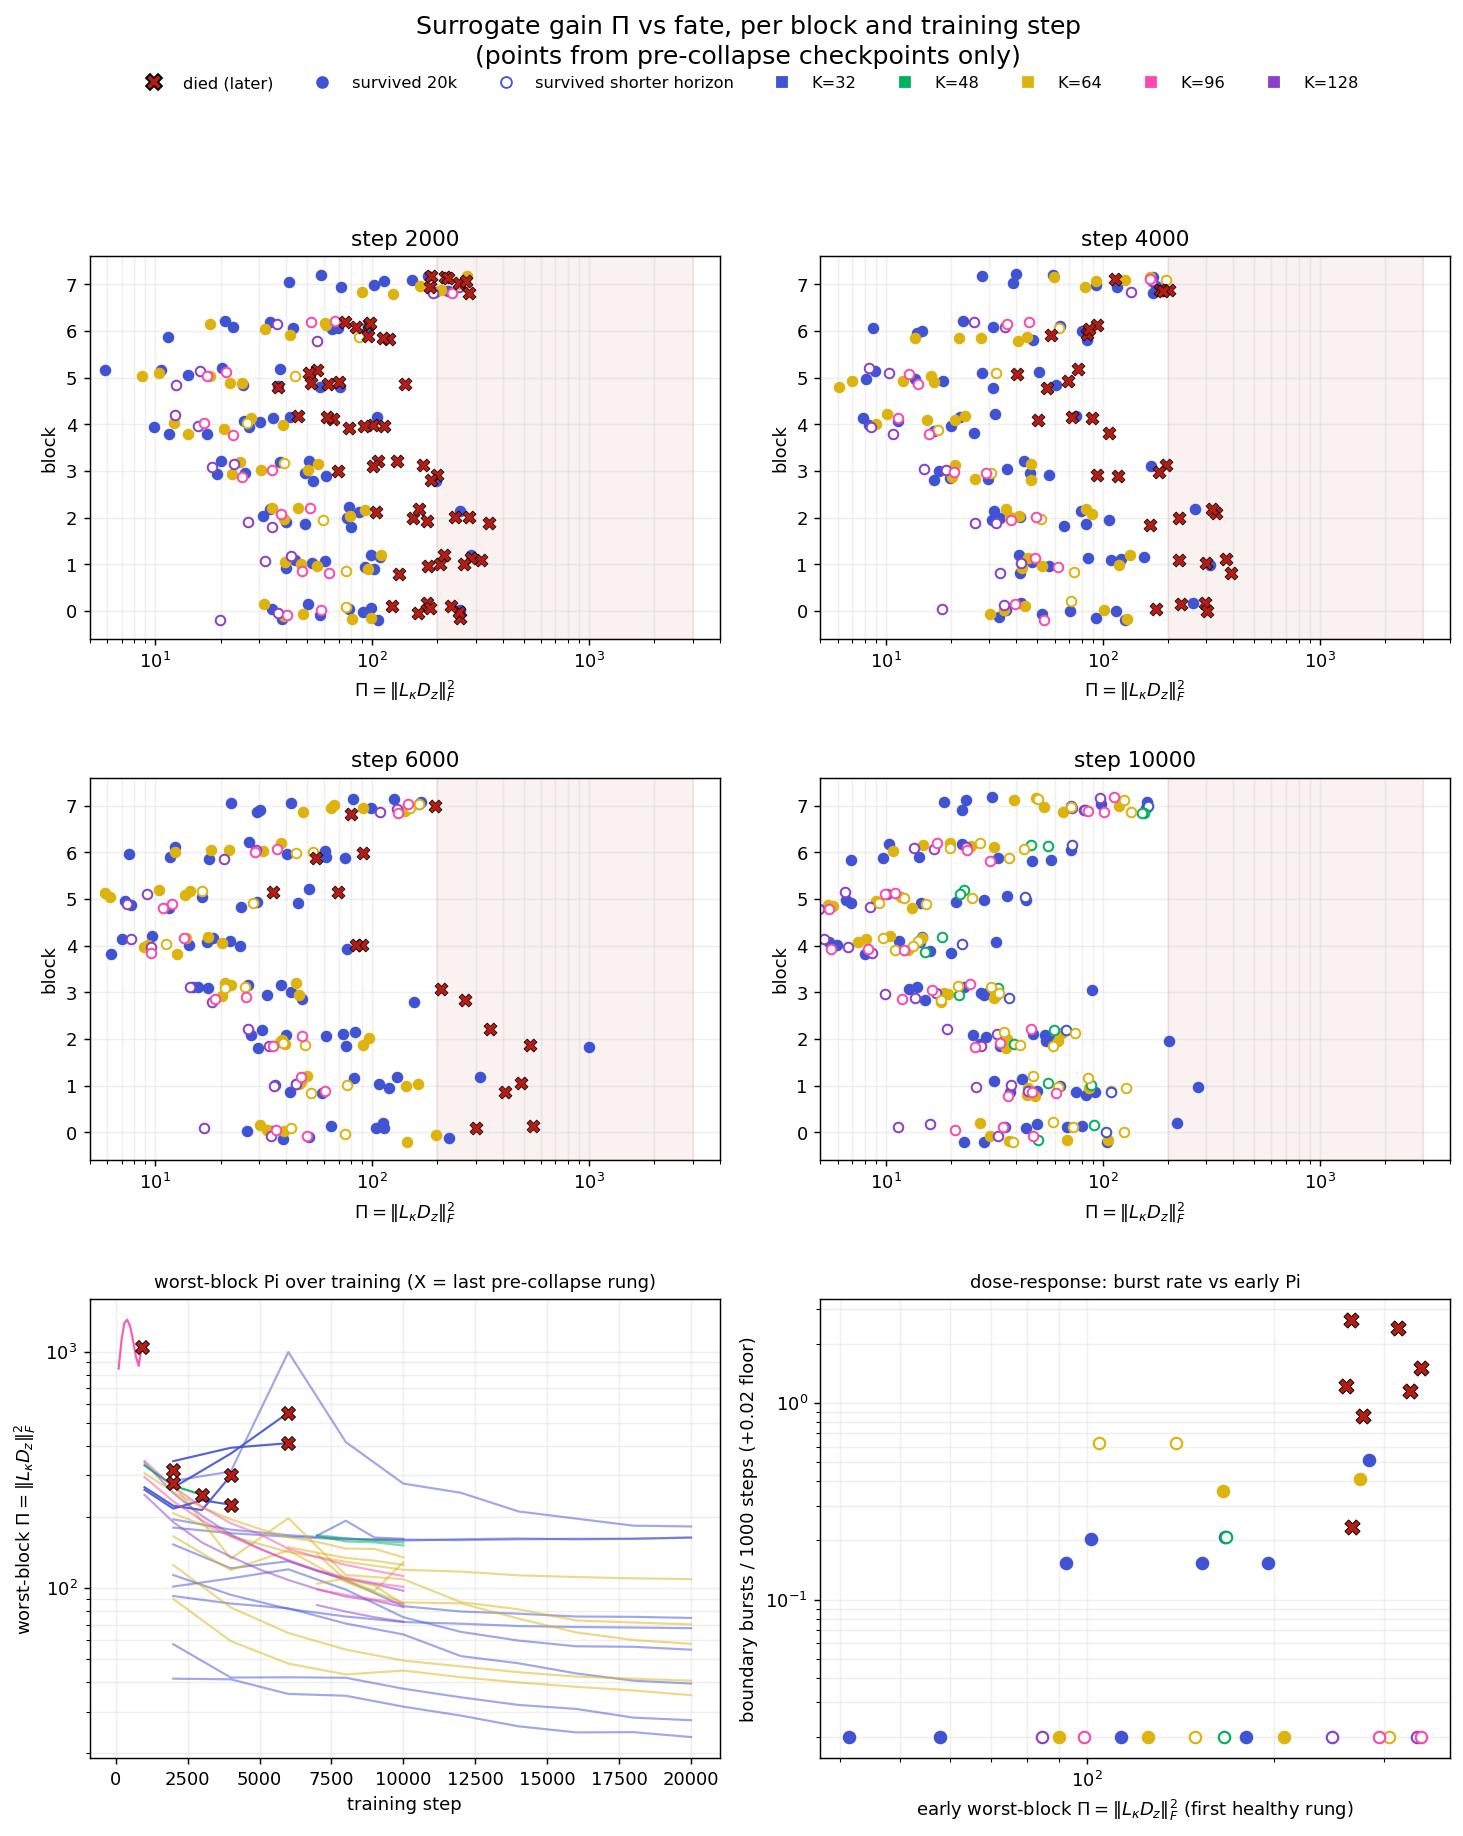
\includegraphics[width=.94\textwidth]{figures/sdn_pi_fate_map.png}
\caption{Exact surrogate gain \(\Pisurr\) versus fate, per block and
training step. Deaths separate from survivors within blocks (upper
panels); the worst-block \(\Pisurr\) of every dying run rises toward the
collapse while every survivor's declines over training (lower left; the
one surviving spike-and-return trace is the recoverable burst of the
\(T{=}0.5\) survivor); the pre-onset burst rate is monotone in the early
worst-block \(\Pisurr\) (lower right).}
\end{figure}

\begin{figure}[h]\centering
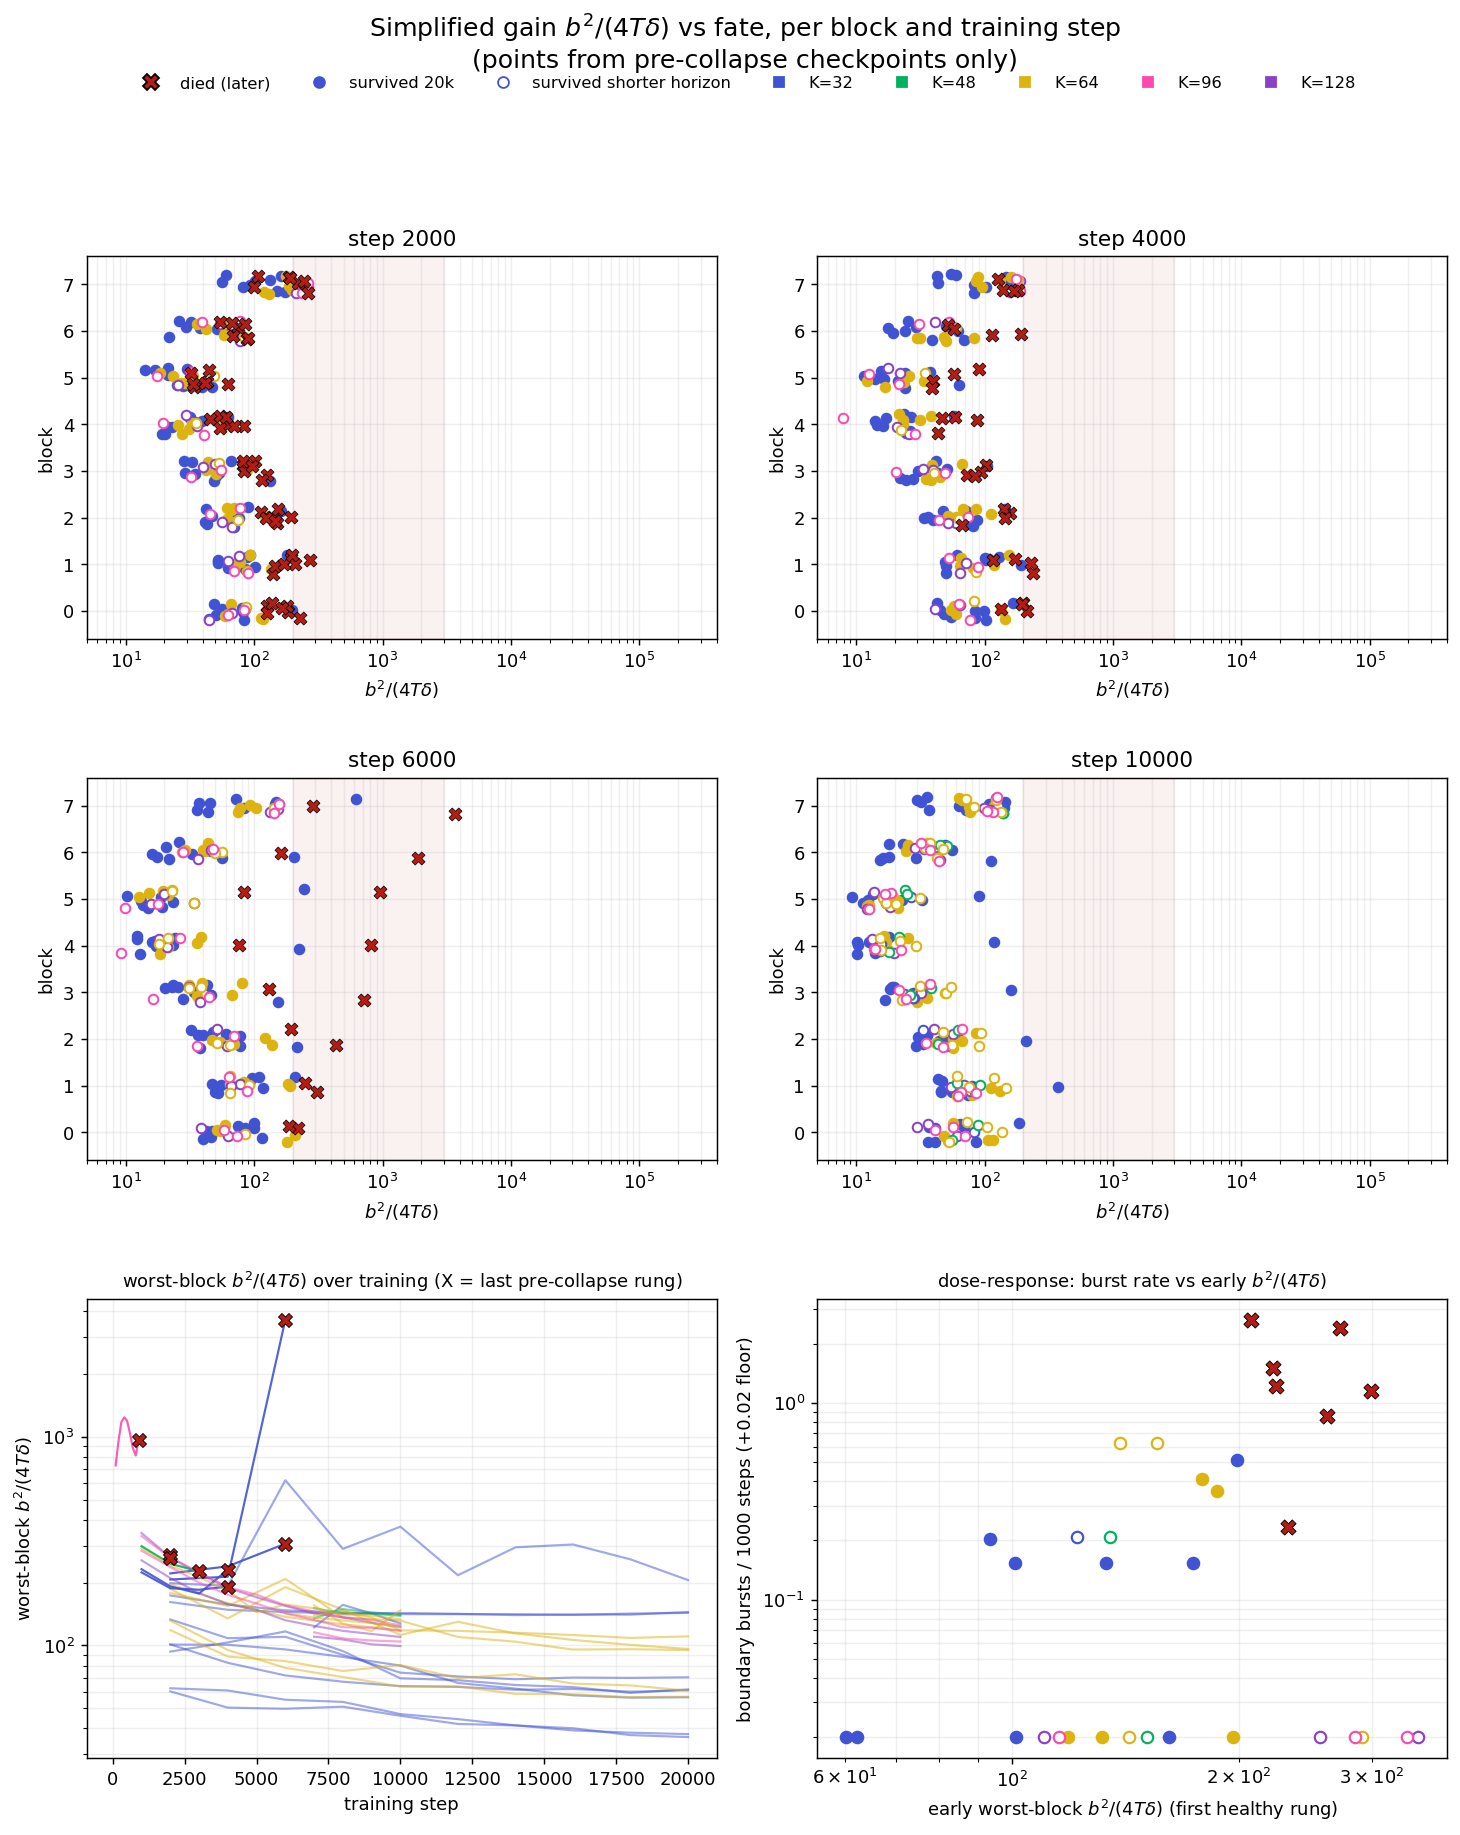
\includegraphics[width=.94\textwidth]{figures/sdn_piapprox_fate_map.png}
\caption{The same construction with the simplified parameter
\(b^2/(4T\delta)\). The dose--response ordering survives, but the
within-block separation is weaker than with the exact \(\Pisurr\) (compare
the step-2000 panels), and individual blocks with collapsing rank spacing
produce far-right outliers; the exact \(\Pisurr\) should be preferred
where the tensors are available.}
\end{figure}

\section{Results 6: drift versus diffusion, and the escape picture}

The learning-rate and batch-size sweeps separate the two destabilization
channels. Signed drift scales approximately linearly and heating
approximately quadratically with the learning-rate multiplier at all three
tested states. At the stable \(k32/T1\) state the heating roughly doubles
when the batch is halved (stochastic, gradient-variance origin); at the
pre-death \(k64/T1\) state it is unchanged (deterministic overshoot of a
large structured gradient). The burst phenomenology of the earlier report
--- recoverable excursions with seed-dependent outcomes --- is reproduced
directly in the marginal continuations (three seeds: one death, two bursty
survivals).

A quantitative Kramers-style collapse of burst rates onto a single escape
number was not achieved with the available data: the restoring-curve slope
\(\lambda\) can be estimated only coarsely (for the calm \(k64/T2\) state,
the surrogate spring crosses zero near \(\alpha \approx 1.4\) with slope
\(\lambda \approx 7\times10^{-3}\) per unit \(\log R\) per step), and only
three \((K,T)\) rows contain both outcomes. The qualitative structure is
nevertheless the escape picture: a scale basin created by restoring drift
(task everywhere; surrogate around its \(T\)-dependent set point), an
excitation source (heating) that grows with the surrogate gain and step
size, and a cliff (window depopulation and correction degeneracy) beyond
which restoration is lost.

\section{Proposed causal sequence for a burst}

Measured facts are marked (M); inference is marked (I).

\begin{enumerate}[leftmargin=1.6em]
\item At marginal pressure the per-step parameter updates near the gate are
large: the surrogate gain \(\Pisurr\) is 3--10 times the calm value (M),
and the total step produces second-order scale heating comparable to or
exceeding the restoring drift at the worst block (M).
\item Heating episodes inflate the score scale of a block; the signed
drifts (task and surrogate) oppose the inflation (M). Most excursions are
therefore recovered (M: continuation replicas; earlier campaign
trajectories).
\item During a large excursion the kernel window thins
(\(\neff\) falls; M in the \(T{=}0.1\) anatomy and prospectively:
low \(\neff\) is the best within-row burst predictor), which concentrates
the correction and raises the per-member gain further (I, consistent with
the \(\Pisurr\) formula).
\item If the excursion reaches the near-degenerate regime, the distributed
correction is lost (\(\Pisurr \to 0\) at \(\neff = 1\), M) while
neighbouring near-degenerate blocks acquire enormous gain
(\(\Pisurr \sim 10^{12}\), M); the remaining surrogate pumps scale
(M: support-off stops it) and the task gradient alone cannot restore the
model while the surrogate is active (M).
\item The runaway propagates through depth by the residual-replacement
composition (earlier report) and terminates in a frozen high-scale state
(M).
\end{enumerate}

\section{Recommended controller variables}

\begin{itemize}[leftmargin=1.4em]
\item \textbf{Fast guard: per-block window population} (equivalently
\(\neff\)). It is the best within-row early warning (AUC 0.75), it is the
variable whose collapse defines the cliff, and the existing servo's
population floor acts on exactly this quantity. The measured refinement:
the guard must never \emph{raise} \(T\) after a block has already
collapsed; at that stage the correct action is to disable the support
gradient (support scale to zero) until the scale statistics recover.
\item \textbf{Pressure gauge: \(\Pisurr\)} (per block), or its forward-only
approximation \(b^2/(4T\delta)\). It is dimensionless,
reparameterization-invariant, tracks the realized gain, and dominates the
pooled prospective comparison. A trim that holds \(\Pisurr\) at a safe
target is the natural upgrade of the current \(\chigeo\)-servo; within this
architecture the two co-move (which is why the \(\chigeo\)-servo works),
but \(\Pisurr\) is the quantity with a mechanistic meaning.
\item \(\chigeo\) should be treated as a convenient row-level heuristic
only.
\end{itemize}

The central question --- what measurable quantity directly indicates that
the score scale is about to become self-amplifying --- has a two-level
answer. The direct indicator is the one-step heating-to-restoration ratio
at the worst block, measurable by the antithetic counterfactual probe
(\code{analysis/scale\_dynamics.py drift}); values approaching one from
below precede collapse (0.02 at calm states, 0.7--1.8 at states that died
within 2000 steps, \(\sim\)2 at 100 steps before death). The cheap
forward-only pair that tracks it is (\(\Pisurr\), \(\neff\)) per block:
\(\Pisurr\) sets the step size the surrogate injects (hence the heating,
which grows quadratically with it), and \(\neff\) measures the distance to
the degeneracy cliff. \(\chigeo\) predicts neither within a row; its
apparent usefulness came from co-moving with \(\Pisurr\) across rows.

\section{Remaining uncertainties and next experiments}

\begin{itemize}[leftmargin=1.4em]
\item The heating term was identified as the destabilizing coupling, but
its propagation constant --- how much one block's heating raises the next
block's scale within one step --- was not measured; a block-resolved
transfer measurement would close this.
\item The one-step counterfactuals do not equal sustained closed-loop
rates: the optimizer's second-moment adaptation tempers repeated large
steps. Short-horizon (10--50 step) branch continuations from the same
states would quantify the closed-loop attenuation.
\item The within-row comparison rests on three \((K,T)\) rows; the
interrupted fate-mapping campaign (16 configurations bracketing the
boundary) would make the prospective table decisive.
\item A \(\Pisurr\)-targeted servo variant has not been run; the
recommendation above predicts it matches or improves on the
\(\chigeo\)-servo and transfers across score reparameterizations by
construction.
\item The escape-rate collapse (\(E_{\mathrm{escape}}\)) remains
unresolved for lack of matched \((\lambda, D, x_c)\) estimates across
enough marginal configurations.
\end{itemize}

\end{document}
